\documentclass[12pt]{article}
\usepackage{latexsym}
\usepackage{amssymb,amsmath}
\usepackage[pdftex]{graphicx}
\usepackage{epstopdf}


\topmargin = 0.1in \textwidth=5.7in \textheight=8.6in

\oddsidemargin = 0.2in \evensidemargin = 0.2in


\begin{document}

\begin{center}
COMPUTER SCIENCE 20, SPRING 2014 \\
Homework Problems\\
Recursive Definitions, Structural Induction, States and Invariants\\
Author: Tawheed Abdul-Raheem
\end{center}

\smallskip

%\subparagraph*{Note:}
%Use the following definition of the set of valid integer binary trees $T$.
%\begin{itemize}
%\item \textbf{Base Cases:} $$\epsilon \in T$$
%\item \textbf{Constructor Case:} If $x \in \mathbb{Z}$, $l \in T$, $r \in T$, then
%$$(x,l,r) \in T$$
%\item A \textit{node} of a tree is any element in $T$ that is a three-tuple, that is, it is of the form $(x,l,r)$. This means that $\epsilon \in T$ is not a node.
%\item If $z = (x,l,r)$ is a node, then $l$ and $r$ are child nodes of $z$, if they are non-empty.
%\end{itemize}
\begin{enumerate}
\item The nodes in a tree obey the \textit{heap property} if, for every node $z$ in the tree, the value in $z$, that is $x$, is at least as big as the value in each of $z$'s children (the tree in module 15 obeys the heap property).\\\\
Prove that if a binary tree has the heap property, then the value in the root of the tree is at least as large as the value in any node of the tree. \\\\
\textbf{Base case: } When the tree has only one node, this means that the child node of this node is $\epsilon$ so it must mean that it is biggest node \\
\textbf{Constructor Case: } In a tree with n-nodes, the root is at least greater or equal to the child nodes.\\
By the definition of the \textit{heap property}, lets assume that there is a new node call it $a$ if node $a$ is greater than the root node of the tree you would swap it with the root node and move the old root to be a child of $a$. On the other hand if $a$ is less than or equal to the root node, you would simply preserve the root node and make $a$ a child node. This will gurantee that each root node would be at least greater or equal to its child nodes.

\item A \textit{complete} binary tree (example below) is a binary tree in which every level, except possibly the last level, is completely filled, and all nodes are as far left as possible.
\begin{center}
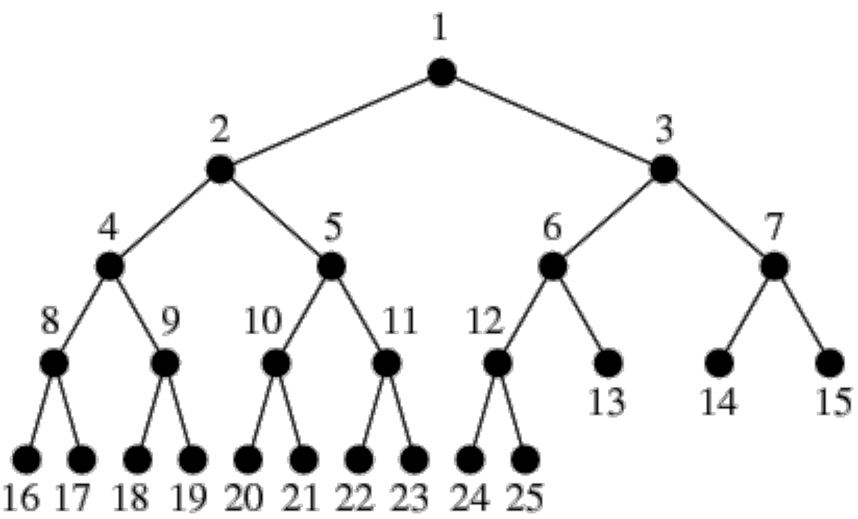
\includegraphics[scale=.3]{CompleteBinaryTree.pdf}
\end{center}
Also, remember that an \textit{internal node} is a node that has children.\\\\
Prove that the number of internal nodes in a complete binary tree with $n$ nodes is $\lfloor n/2 \rfloor$ where $\lfloor x \rfloor$ equals the largest integer that is not greater than $x$. \\\\
\textbf{Base case: } $1$-node tree. The children of a \textit{1 node tree} is $\epsilon$ \\
\textbf{Constructor case: } For all trees with depth $\le k$, if the number of nodes is $n$, then the number of internal nodes is $\lfloor n/2 \rfloor$\\
Lets say that we have a tree of depth $k+1$, and also with $l$ left nodes and $r$ right nodes, the height of the internal node of the tree would be its left side, right side as well at its depth. $\forall \text{ binary tree the number of internal node is }$
$ \lfloor left/2 \rfloor + \lfloor right/2 \rfloor + 1$
\item (From Meyer, problem 6.6) Let $m,n \in \mathbb{Z}$ where $m \not = 0$ and $n \not = 0$. Then, let's define a set of integers, $L_{m,n}$, recursively as follows:
\begin{itemize}
\item \textbf{Base cases:} $m,n \in L_{m,n}$
\item \textbf{Constructor cases:} If $j,k \in L_{m,n}$, then
\begin{enumerate}
\item $-j \in L_{m,n}$. and
\item $j + k \in L_{m,n}$
\end{enumerate}
\end{itemize}
Let $L$ be an abbreviation for $L_{m,n}$ for the rest of this problem.
\begin{enumerate}
\item Prove by structural induction that every common divisor of $m$ and $n$ also divides every member of $L$. \\
    Assume every other element is divisible by $k$ and assume by contradiction that new element $k$ is not divisible by $k$, but this is impossible because $x$ is
    generated by the negation or $i+j$ where $i$ and $j$ are both old elements of the set, therefore they must be divisible by $k$
\item Prove that any integer multiple of an element of $L$ is also in $L$.\\
    Lets say $x$ is an integer, $x \in L_{m,n}$, we also know that $-j \in L_{m,n}$ As the easiest multiple of a number is $1 \cdot $ the number itself. We can say that the multiple of the negation of $x$ is a multiple that also exists in $L$ 
\item Show that if $j,k \in L$ and $k \not = 0$ then the remainder of $j$ divided by $k$ is also in $L$; that is, that  $\mathsf{rem}(j,k) \in L$. \\
    If we have that $L_{4,12} \in \{4,12,-4,-12,0,8,16,-8,-16,-24, ... \}$ \\
    We see that $12 \text{and} 4$ are both in $L$\\
    $\mathsf{rem}(4,12)$ is $4$ which happens to also be in set $L$
\end{enumerate}
\item (From Sipser, exercise 1.6) Draw state machines that only accept strings in the following set. Assume that the alphabet is $\Sigma = \{0,1\}$; that is, that all strings $s \in \Sigma^*$.\\ (Bonus point(s) if you draw your raw state machines in LaTeX; check out the TikZ package to do this.)
$$\{w:w \text{ contains the substring 0101, i.e. }w = x0101y \text{ for some }x \text{ and }y\}$$
\textbf{Steps Involved: } This is the steps that happens for the input string \\
\textbf{Step 1: } If the first input is a 1 loop\\
\textbf{Step 2: } If the first input is a 0 move to next state\\
\textbf{Step 3: } If it is a 0 go to step 2 else move on to the next state\\
\textbf{Step 4: } If it is a 1 go to step 2 else move to the next state\\
\textbf{Step 5: } If it is a 0 go to step 2 else move to next state\\
\textbf{Step 6: } If we get here, we have found our string so terminate\\
    \begin{center}
    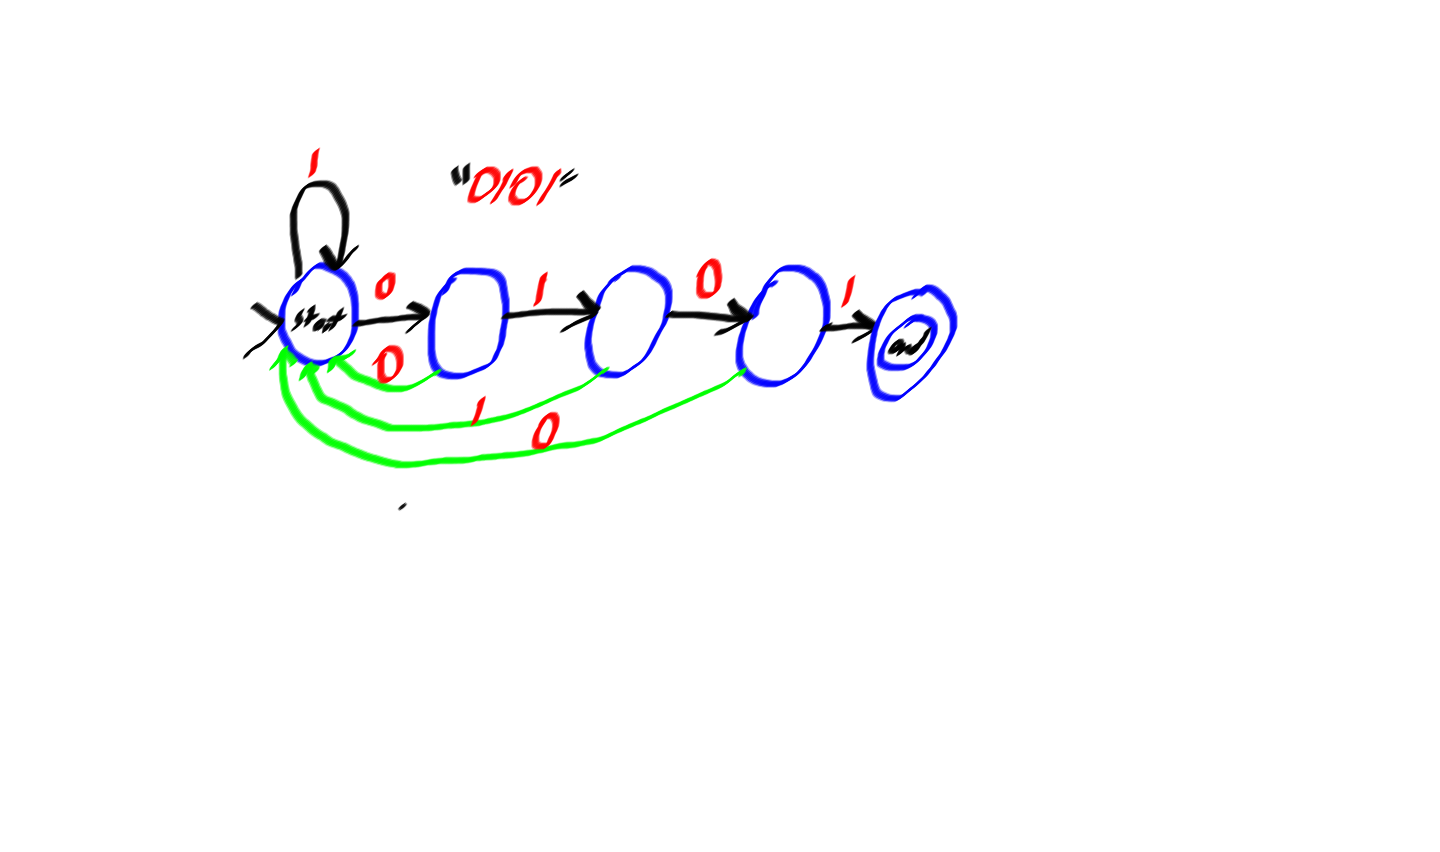
\includegraphics[scale=0.25]{state_machine.png}
    \end{center}
\item (From Meyer, problem 5.29) A robot named Wall-E wanders around a two-dimensional grid. He starts at (0,0) and is allowed to take four different types of steps:
\begin{enumerate}
\item (+2,-1)
\item (+1, -2)
\item (+1, +1)
\item (-3, 0)
\end{enumerate}
For example, Wall-E might take the following stroll. The types of his steps are denoted by each arrow's subscript:
$$(0,0) \to^a (2,-1) \to^c (3,0) \to^b (4,-2) \to^d (1,-2) \to \ldots$$
Wall-E's true love, the fashionable and high-powered robot, Eve, awaits at (0,2).
\begin{enumerate}
\item Describe a state machine model of this problem. \\\\
    Based on the possible steps that was given in the problem, we know that Wall-E can take either negative or positive steps. For every move that Wall-E makes we can see that the sum of the numbers that does not change is $\pm 1$  and $\pm 2$ \\
    \textit{P(n) } := if $q$ is a state reachable in $n$ transitions, then $q$ must either be $\pm 1$ or $\pm 2$ \\
    \textbf{base case:} P(0) since the only state reachable in 0 transitions is the start state (0,0) our claim holds\\
    \textbf{inductive step: } Assume that $P(n)$ is true and let $r$ be any state reachable in ... transitions. We need to prove the lemma.
    Since $r$ is reachable in a multiple of 2 transitions, there must be a state ,$q$, reachable in $n$ transitions such that $q \to r$. Since $P(n)$ is assumed to be true, the claim holds. This proves that $P(n)$ IMPLIES $P(2n)$ as required completing the proof of the inductive step. We conclude by the induction that for all $\pm 2n$, if $q$ is reachable in $n$ transitions. Then our claim is true.
\item Will Wall-E ever find his true love? Either find a path from Wall-E to Eve or use the Invariant Principle to prove that no such path exists. \\\\
    Wall-E will never find his true love, see picture below:
    \begin{center}
    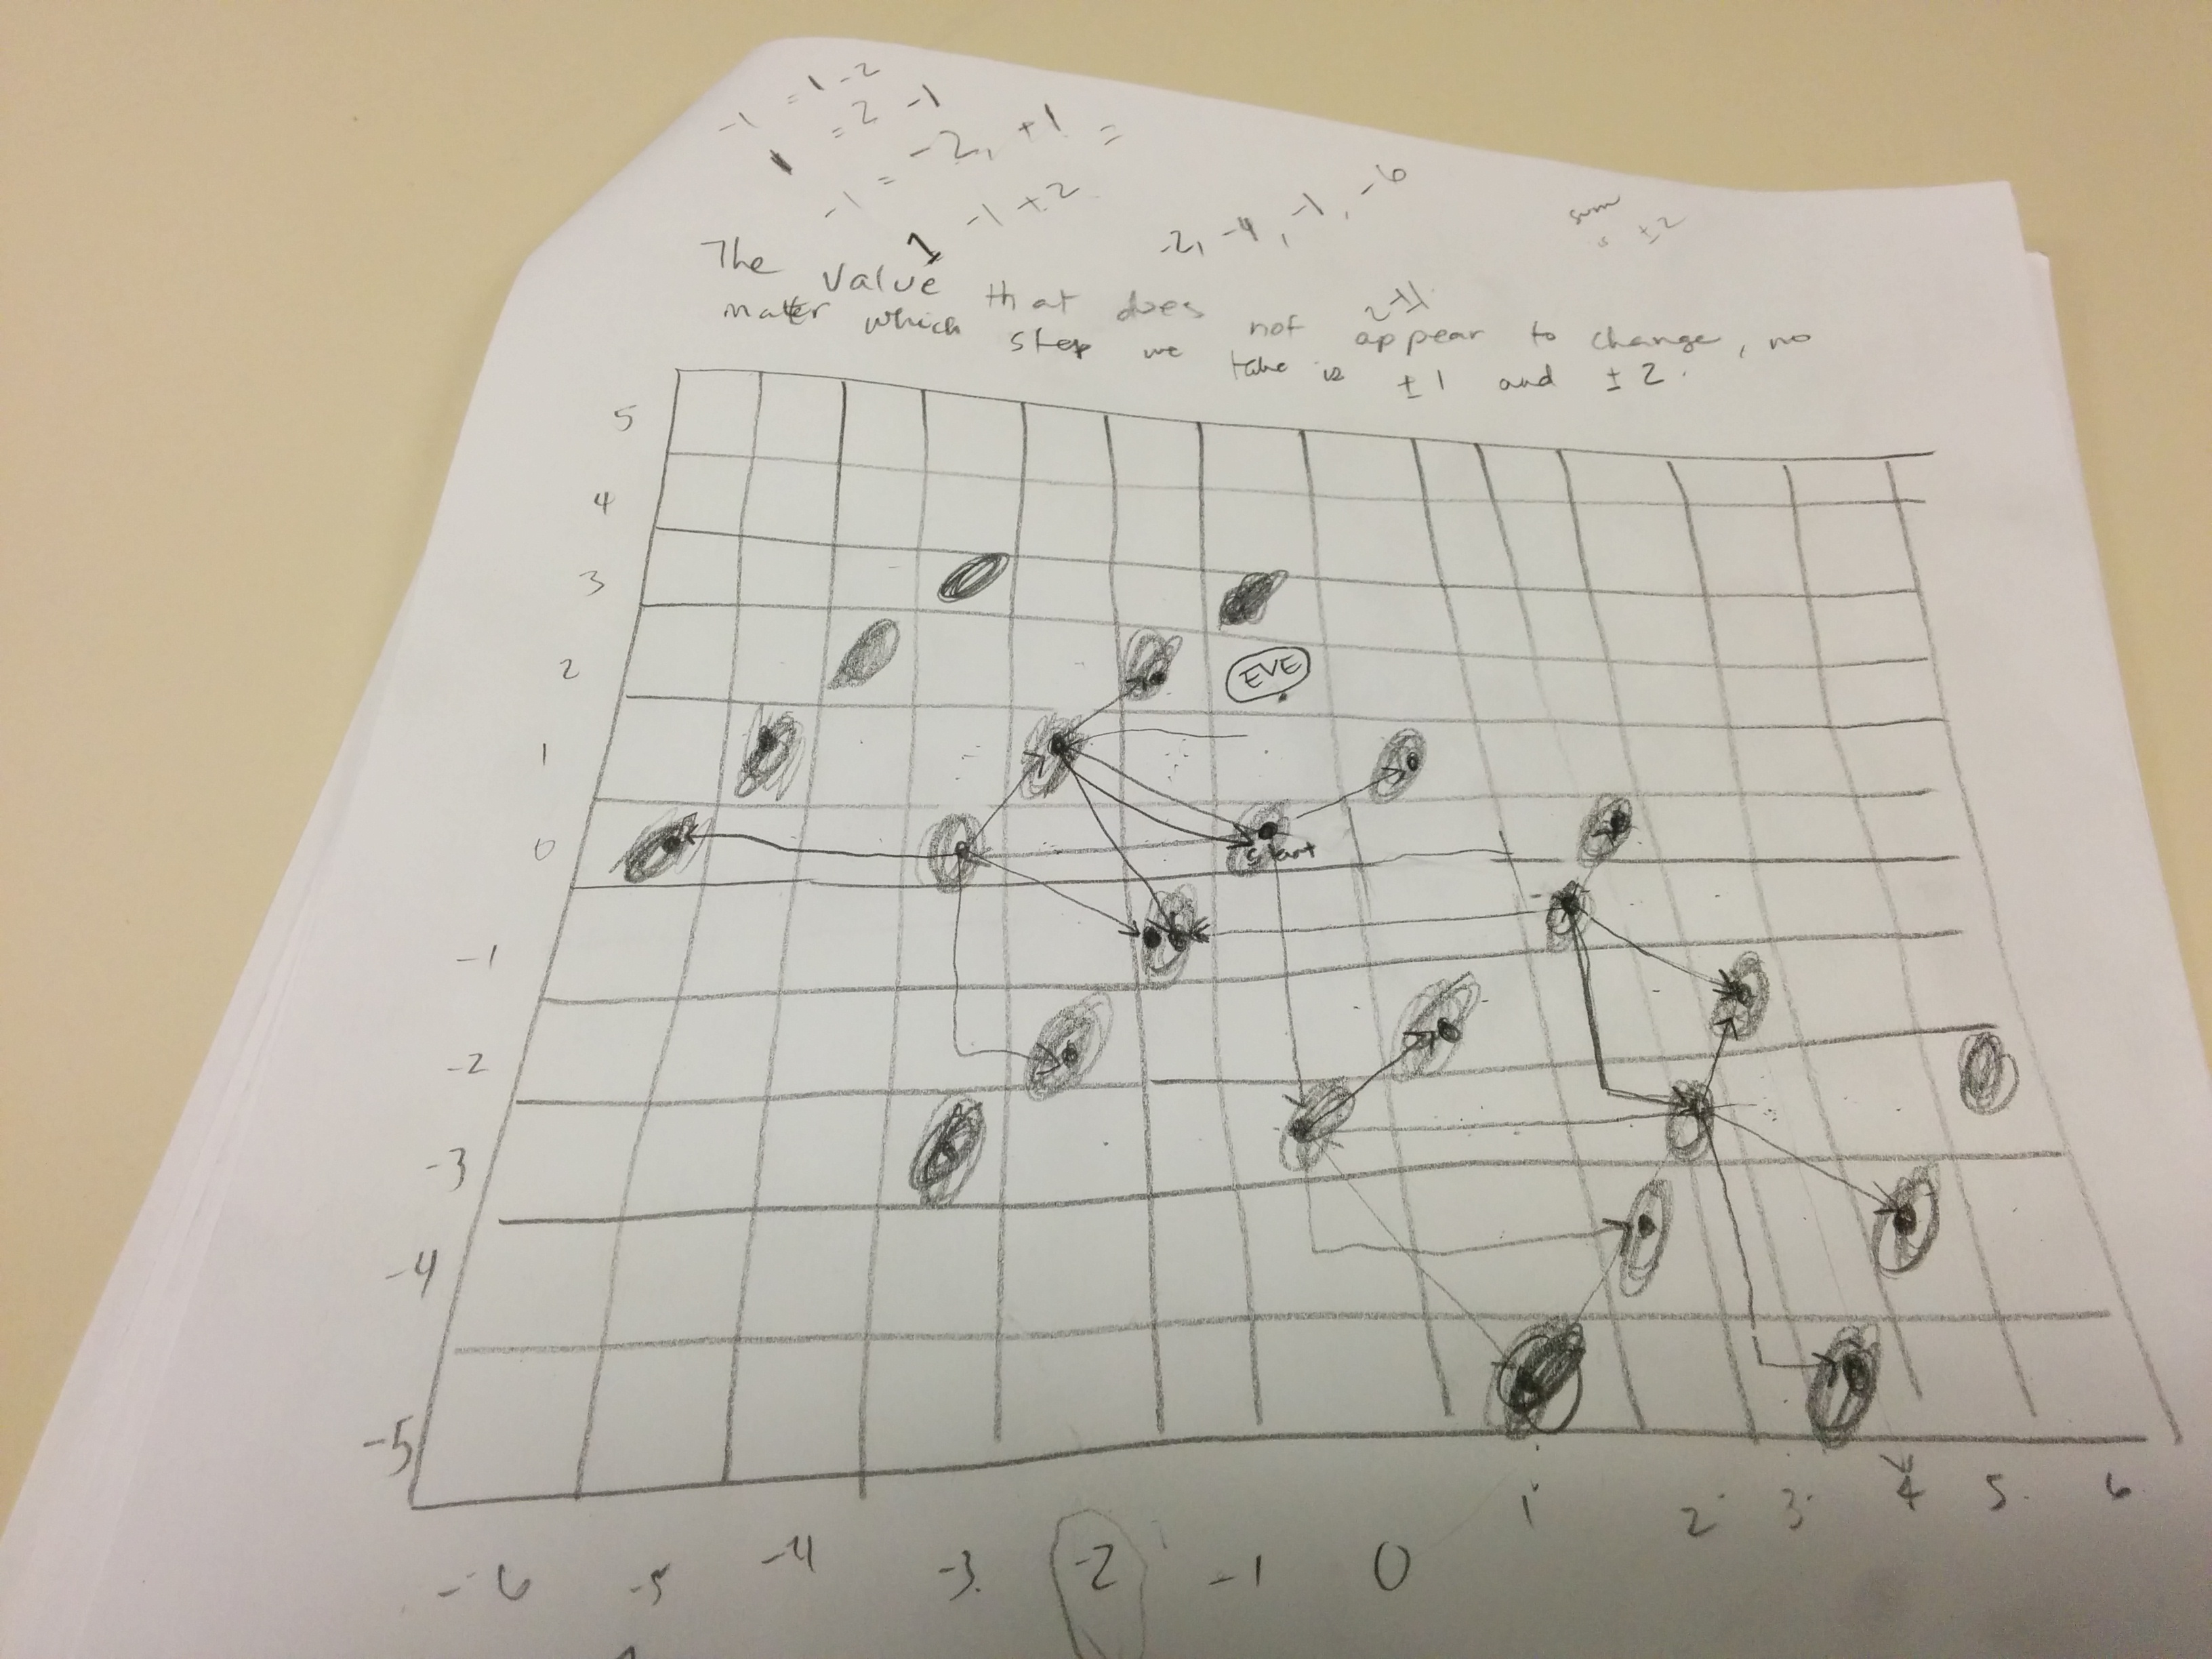
\includegraphics[scale=0.10]{walle.jpg}
    \end{center}
\end{enumerate}
\end{enumerate}
\end{document}
